\documentclass[11pt]{article}

\usepackage[a4paper,margin=1in]{geometry}
\usepackage[T1]{fontenc}
\usepackage[utf8]{inputenc}
\usepackage{mathptmx}
\usepackage{microtype}
\usepackage{booktabs}
\usepackage{graphicx}
\usepackage[round]{natbib}
\usepackage{hyperref}
\usepackage{url}
\usepackage{amsmath}
\usepackage{xcolor}
\usepackage{enumitem}
\usepackage{authblk}
\newcommand{\num}[1]{#1}
\setlist{itemsep=2pt,topsep=4pt}
\setlength{\emergencystretch}{3em}
\hypersetup{colorlinks=true,linkcolor=black,citecolor=blue!50!black,urlcolor=blue!50!black}

\title{\textbf{Boundary-Aware Token-Structure Analysis of the Voynich Manuscript:\\
A Reproducible Reassessment}}
\author[1]{Amy Laird\thanks{ORCID: \url{https://orcid.org/0009-0001-5479-0007}}}
\affil[1]{Independent Researcher \\ \texttt{laird2214@gmail.com}}
\date{July 2026}

\begin{document}
\maketitle

\begin{abstract}
The Voynich Manuscript (Beinecke MS~408) is a fifteenth-century codex
written in an undeciphered script. We analyze token-family transitions and
automatically discovered prefix and suffix families in the frozen
Zandbergen--Landini EVA transcription (\num{31608} tokens in \num{4197}
lines on 184 pages). This revision replaces earlier analyses that flattened
sequence boundaries or used unmatched comparator sizes. Under a canonical
prefix-first classifier and strictly within Voynich lines,
CHEDY$\to$QOK occurs 615 times, or $2.659\times$ its independence
expectation, while AIIN$\to$QOK occurs 127 times, or $0.444\times$
expectation. These are descriptive transition-matrix effects; matrix-wide
cluster-aware inference remains open. Raw \texttt{aiin}/\texttt{ain}
substring density has similar observed means in Currier A and B pages, but
equivalence was not tested and canonical AIIN-family density differs between
the groups.

The central cross-corpus analysis applies identical automatic affix discovery
to Voynich and every comparator, preserves lines and sentences, resamples
Voynich by page blocks, and repeatedly samples comparator sequence units
without replacement to exactly \num{31608} tokens. Across 200 replicates,
Voynich has median prefix self-clustering $1.333$ (95\% replicate interval
$[1.222,1.461]$), suffix self-clustering $1.458$ ($[1.389,1.555]$), and ratio
$0.918$. Its median minimum-side score is $1.333$. Including the catch-all
\texttt{OTHER} class lowers the corresponding medians to $1.292$, $1.363$,
and $0.951$. Voynich exceeds each of 14 eligible comparators on the continuous
minimum-side score in these sampled distributions; corrected two-sided
replicate sign tests are $p=0.00995$ and remain $0.00995$ after
Benjamini--Hochberg adjustment. This finite-set result does not establish
natural-language uniqueness, language identity, decipherment, or exclusion
of constructed, hybrid, stenographic, cipher, or other historical mechanisms.
One declared comparator, Ottoman Turkish, is ineligible because its preserved
sentence corpus contains only \num{16890} usable tokens and is not padded.
\end{abstract}

\noindent\textbf{Keywords:} Voynich manuscript, corpus linguistics,
sequence boundaries, self-clustering, reproducible research, statistical text
analysis.

\bigskip
\noindent\textbf{Scope statement.} This paper measures properties of one
transcription under declared procedures. It does not translate the manuscript,
assign semantic meanings, identify a language, prove natural or encoded
language, or rule out untested mechanisms.

\section{Introduction}

The Voynich Manuscript is a codex of unknown authorship held by Yale's
Beinecke Rare Book and Manuscript Library as MS~408 \citep{Clemens2016}.
Radiocarbon dating places its vellum between 1404 and 1438
\citep{Hodgins2011}. Numerous decipherment proposals have been advanced, but
none has achieved independent verification. A separate line of work treats
the transcription as a corpus and studies its statistical structure without
attempting translation. Prior work has reported non-randomness, Zipf-like
frequency structure, and section-associated vocabulary
\citep{Reddy2011,Montemurro2013,Bowern2021}.

This project belongs to the latter tradition. It asks two limited questions.
First, how do five declared EVA token families transition within manuscript
lines? Second, when prefix and suffix families are discovered by the same
algorithm in every corpus, how do their self-clustering estimates compare in a
fixed set of size-matched corpora?

The present revision follows a technical audit that identified conflicts among
historical scripts, results, tests, and prose. Earlier public versions used
flattened token streams in the prefix/suffix analysis, allowed artificial
adjacency at corpus and resampling seams, used unequal corpus sizes, included
\texttt{OTHER} in the headline mean, and applied a hand-selected Voynich
prefix partition while discovering comparator families automatically. Those
results, including the values $1.52$, $1.54$, and ratio $0.99$, are retired.
The historical files remain archived in the repository rather than being
silently overwritten.

\section{Data and Methods}

\subsection{Frozen Voynich corpus}

The canonical input is the Zandbergen--Landini source within the frozen
\texttt{AncientLanguages/Voynich} parquet snapshot. Canonical tokenization
produces \num{31608} tokens in \num{4197} nonempty lines on 184 pages. SHA-256
hashes for the input and relevant code are recorded in the generated result.
Lines are the natural adjacency units. Pages are the block units for Voynich
uncertainty resampling. No canonical transition is constructed across lines,
pages, sections, hands, removed-token positions, or resampled blocks.

\subsection{Declared EVA families and ambiguity}

The core transition analysis uses five predicates plus \texttt{OTHER}:

\begin{itemize}
  \item QOK: token begins with \texttt{qok};
  \item OK: token begins with \texttt{ok} but not \texttt{qok};
  \item OT: token begins with \texttt{ot};
  \item CHEDY: token contains \texttt{chedy}, \texttt{shedy},
        \texttt{chey}, or \texttt{shey};
  \item AIIN: token contains \texttt{aiin} or \texttt{ain}.
\end{itemize}

These predicates overlap. Exactly 1,423 token instances (4.5020\%; 160
types) match more than one family. The canonical policy gives prefix
predicates precedence in the order QOK, OK, OT, CHEDY, AIIN. A strict
sensitivity policy removes ambiguous tokens and breaks the sequence at every
removed position, so former neighbors never become adjacent. The predicates
are EVA-specific and are not paleographic identifications.

\subsection{Within-line transition estimates}

For a source class $s$ and destination class $d$, the descriptive ratio is
\[
R(s\to d)=\frac{N_{s\to d}}
{N_s^{\mathrm{src}}N_d^{\mathrm{dst}}/N_{\mathrm{transitions}}}.
\]
Counts and marginals are pooled only over transitions that already occur
within separate lines. The permutation null shuffles class labels within each
line, uses 2,000 replicates, and reports the corrected empirical estimate
$(b+1)/(B+1)$ rather than zero. Individual transition cells remain clustered
within lines and pages, so the cell-level permutation values and the ordinary
$6\times6$ independence statistic are treated as descriptive pending a
matrix-wide cluster-aware analysis.

\subsection{AIIN density decomposition}

Two quantities are kept distinct. Raw substring density counts every token
containing \texttt{aiin} or \texttt{ain}. Canonical-family density counts only
tokens assigned to AIIN after precedence resolves overlap. Per-page Currier A
and B distributions are compared with a two-sample Kolmogorov--Smirnov test.
A nonsignificant difference test is not interpreted as proof of equivalence or
invariance.

\subsection{Comparator corpora and sequence units}

The Version~2 comparison declares 12 Leipzig Wikipedia corpora: Arabic,
Latin, Estonian, Hebrew, Finnish, Hungarian, Turkish, Italian, North
Azerbaijani, Swahili, Georgian, and Tagalog. Each Leipzig sentence record is
one sequence unit. Middle English \emph{Canterbury Tales} and KJV English are
frozen Gutenberg documents split into sentence-like units after removing
Gutenberg headers and footers. Ottoman Turkish is read from genuine CoNLL-U
sentence boundaries. Mandarin and pending corpora are not part of this
estimator.

Leipzig texts are modern Wikipedia proxies, not historical or genre-matched
controls. The two Gutenberg texts are historical literary comparators, not
matched manuscript genres. Ottoman Turkish provides only \num{16890} usable
tokens under preserved sentence boundaries, below the target \num{31608}, and
is therefore declared ineligible. It is neither flattened nor padded.

\subsection{Matched resampling}

Each eligible comparator replicate randomly orders natural sequence units
without replacement and takes whole units until reaching the exact target of
\num{31608} tokens. If the final unit would overshoot, a random contiguous
fragment supplies the remaining tokens and remains a separate sequence.
Voynich uncertainty is estimated with page-block bootstrap replicates. A
sampled page contributes its original separate lines; a final partial line is
a separate contiguous fragment. These procedures cannot create adjacency
across sentence, document, line, page, sample, or truncation boundaries.

The analysis uses 200 replicates and master seed \texttt{20260718}. Every
child seed is recorded. Replicate intervals are percentile summaries of the
declared resampling distributions, not guarantees about an unobserved
population of all languages or transcriptions.

\subsection{Symmetric affix discovery and self-clustering}

For each system and replicate, the same discovery procedure is applied
separately to prefixes and suffixes. Candidate affixes have length two or
three code points, cover 2\% through 20\% of tokens, and are selected from the
80 most frequent candidates. Selection is greedy with lexical tie-breaking;
nested candidates on the same side are excluded; at most five families are
retained. Each token is assigned to the first selected family it matches or to
\texttt{OTHER}.

For discovered class $c$, self-clustering is observed within-unit
$c\to c$ divided by the expectation from pooled within-unit source and
destination marginals. A class enters the unweighted mean when both marginals
exceed 10 and its expected self-transition count exceeds one. The primary
score excludes \texttt{OTHER}. Including \texttt{OTHER} is a required
sensitivity condition. Primary continuous outcomes are prefix score $P$,
suffix score $S$, ratio $P/S$, and balanced elevation $\min(P,S)$.

Bucket labels are secondary. Threshold sensitivity crosses elevation
thresholds 1.05, 1.10, and 1.15; ratio lower bounds 0.75, 0.80, and 0.85; and
upper bounds 1.20, 1.25, and 1.30, for 27 cells.

For each eligible comparator, replicate-wise differences in $\min(P,S)$ are
summarized by their median and percentile interval. A corrected two-sided
replicate sign estimate is reported and adjusted by Benjamini--Hochberg over
the 14 eligible comparator tests. The smallest possible two-sided corrected
value with 200 replicates is $2/(200+1)=0.00995$.

\subsection{Reproducibility and source hierarchy}

The canonical hierarchy is shared code, frozen inputs and manifests,
pipeline-listed scripts, fresh generated results, tests, current prose, the
paper, and finally archived analyses. Generated outputs override prose. The
command \texttt{python run\_all.py} validates inputs, regenerates the core and
prefix/suffix analyses, runs pytest and direct Python execution, checks output
freshness, and writes a run manifest. Estimator version, command, input and
code hashes, Git revision, and seeds are stored in
\texttt{results/prefix\_suffix\_v2.json}.

\section{Results}

\subsection{Within-line transition structure}

Under canonical precedence and strictly within lines, CHEDY$\to$QOK has
615 observations against an expectation of approximately 231, giving
$R=2.659$. AIIN$\to$QOK has 127 observations against an expectation of
approximately 286, giving $R=0.444$. Both corrected within-line shuffle
values are $p=0.0005$. CHEDY$\to$QOK spans 312 unique canonical within-line
token pairs. Among 58 sufficiently frequent CHEDY token types, 44 (76\%)
meet the project's declared attraction criterion.

These estimates establish class-level departures from the independence
baseline in this representation. They do not by themselves establish syntax,
semantics, or independence of transition events. The ordinary matrix
statistic is therefore not used to make individual confirmatory cell claims.

\subsection{AIIN is not canonically invariant}

Raw \texttt{aiin}/\texttt{ain} substring density has observed page means of
approximately 15.0\% in both Currier A ($n=102$ pages) and B ($n=72$), with
KS $p=0.742$. The difference procedure did not reject equality, but no
equivalence margin or equivalence test was specified. The appropriate result
is descriptive similarity, not invariance.

After canonical precedence resolves overlapping families, mean AIIN-family
density is 13.58\% in Currier A and 10.77\% in Currier B, with KS
$p=0.0028$. Thus the earlier broad claim that AIIN-family density is invariant
is rejected. Raw substring occurrence and canonical assignment answer
different questions and must not be substituted for one another.

\subsection{Boundary-aware prefix/suffix comparison}

Table~\ref{tab:comparison} reports primary medians. Voynich has prefix score
1.333, suffix score 1.458, ratio 0.918, and minimum-side score 1.333. The
prefix and suffix 95\% replicate intervals are $[1.222,1.461]$ and
$[1.389,1.555]$, respectively.

\begin{table}[ht]
\centering
\small
\caption{Version~2 primary estimates. All eligible systems are repeatedly
matched to \num{31608} tokens. $\Delta\min$ is Voynich minus comparator;
brackets give its 95\% replicate interval. \texttt{OTHER} is excluded.}
\label{tab:comparison}
\begin{tabular}{lrrrrl}
\toprule
System & Prefix & Suffix & $P/S$ & $\min(P,S)$ & $\Delta\min$ [95\% interval] \\
\midrule
\textbf{Voynich} & \textbf{1.333} & \textbf{1.458} & \textbf{0.918} & \textbf{1.333} & target \\
Arabic & 1.485 & 0.877 & 1.693 & 0.877 & 0.456 [0.285, 0.644] \\
Latin & 0.543 & 2.642 & 0.206 & 0.543 & 0.767 [0.476, 0.963] \\
Estonian & 0.701 & 1.939 & 0.362 & 0.701 & 0.622 [0.451, 0.843] \\
Hebrew & 0.565 & 1.707 & 0.331 & 0.565 & 0.768 [0.402, 1.000] \\
Finnish & 0.622 & 1.395 & 0.446 & 0.622 & 0.713 [0.532, 0.891] \\
Hungarian & 0.546 & 0.659 & 0.829 & 0.544 & 0.791 [0.660, 0.931] \\
Turkish & 0.619 & 0.779 & 0.795 & 0.615 & 0.719 [0.548, 0.875] \\
Italian & 0.604 & 0.810 & 0.746 & 0.604 & 0.725 [0.605, 0.871] \\
N. Azerbaijani & 0.714 & 0.840 & 0.850 & 0.704 & 0.627 [0.416, 0.808] \\
Swahili & 0.819 & 0.998 & 0.821 & 0.819 & 0.513 [0.399, 0.643] \\
Georgian & 0.985 & 0.812 & 1.213 & 0.811 & 0.520 [0.377, 0.670] \\
Tagalog & 0.467 & 0.615 & 0.759 & 0.467 & 0.864 [0.745, 0.996] \\
Middle English & 0.338 & 0.400 & 0.845 & 0.336 & 0.994 [0.879, 1.133] \\
KJV English & 0.259 & 0.094 & 2.755 & 0.094 & 1.234 [1.130, 1.373] \\
\bottomrule
\end{tabular}
\end{table}

All 14 primary $\Delta\min$ distributions are positive at their reported
2.5th percentiles. Each corrected two-sided replicate sign estimate is
$p=0.00995$; because all raw values tie, Benjamini--Hochberg adjustment leaves
them at 0.00995. This resolution is determined by the 200-replicate design.
It should not be reported as stronger evidence than the design permits.

The minimum-side result is not equivalent to saying that both Voynich side
scores exceed both comparator side scores. For example, Latin has much higher
suffix clustering, and Arabic has higher median prefix clustering. The result
instead says that Voynich has the larger weaker-side score in the finite
tested set under this estimator.

\begin{figure}[ht]
\centering
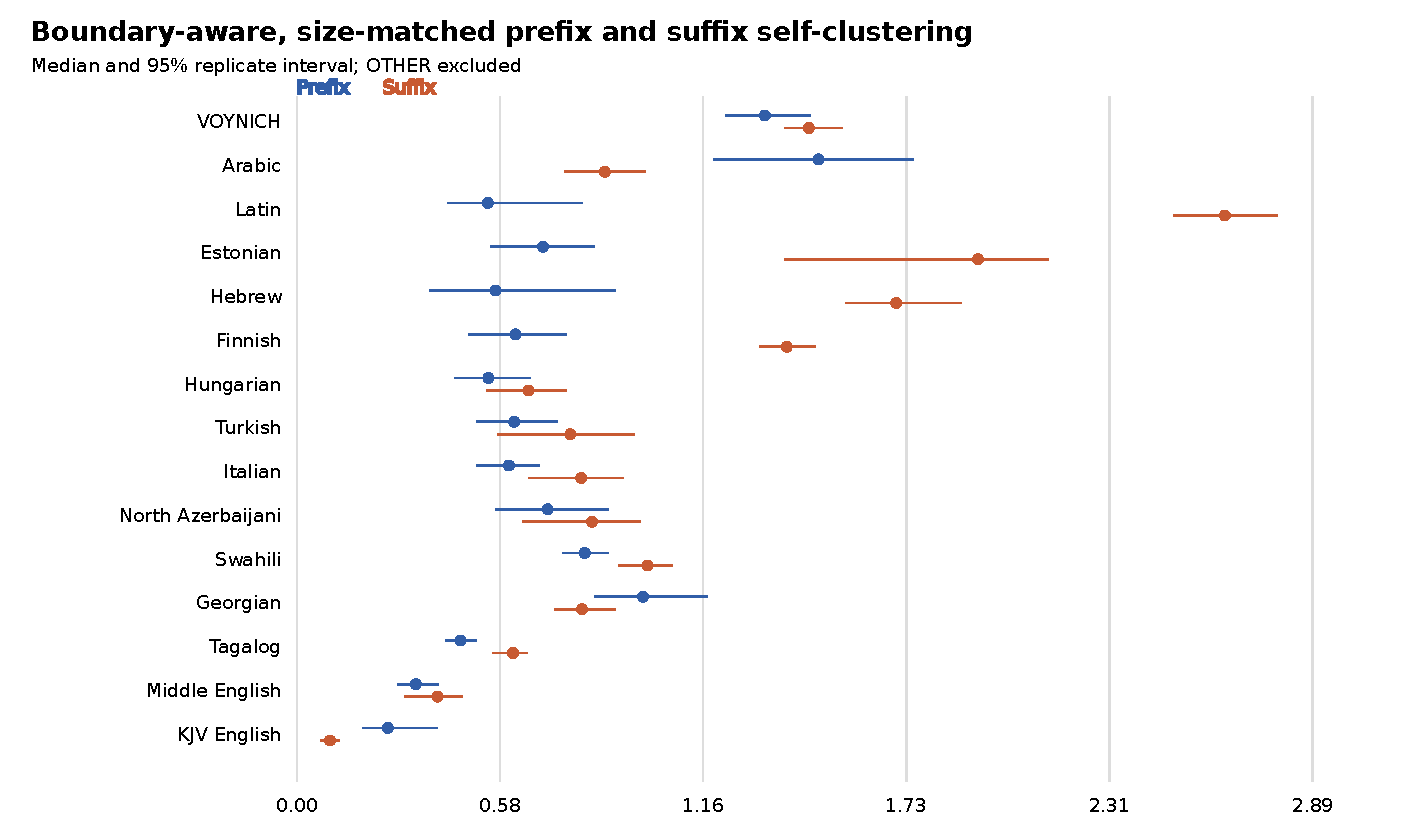
\includegraphics[width=0.96\linewidth]{figures/prefix_suffix_v2.pdf}
\caption{Programmatically generated median prefix and suffix self-clustering
with 95\% replicate intervals. Natural sequence boundaries are preserved and
all eligible samples are matched to \num{31608} tokens.}
\label{fig:v2comparison}
\end{figure}

\subsection{Sensitivity to \texttt{OTHER} and thresholds}

Including \texttt{OTHER} in the class mean changes the Voynich medians to
prefix 1.292, suffix 1.363, ratio 0.951, and minimum-side 1.291. The effect
remains elevated but is smaller, which confirms that the catch-all class is a
material estimator choice and should not be hidden in the headline mean.

Under the 27 declared bucket definitions, Voynich is labeled
\texttt{SYMM-HIGH} in 89\% to 100\% of replicates, depending on thresholds.
This is evidence of threshold robustness within the declared grid, not an
invariant categorical identity. Continuous estimates remain primary.

\subsection{Retractions and narrowed findings}

The audit produced the following claim changes relevant to this paper:

\begin{itemize}
  \item The prefix 1.52, suffix 1.54, ratio 0.99 comparison is retired. It
        came from a boundary-crossing, unmatched, asymmetric estimator.
  \item ``Unique among natural languages'' is retired. The defensible result
        is limited to 14 eligible frozen comparators and the Version~2 method.
  \item Canonical AIIN-family invariance is rejected. Only raw substring
        density has similar observed Currier A/B means, without an equivalence
        test.
  \item The claimed five-to-ninefold joint-feature compounding is rejected;
        a permutation estimator gives a narrower descriptive range of
        approximately 1.53 to 4.27.
  \item The claim that all five agreement cascades survive the corrected
        procedure is rejected; the July procedure reports four of five, and
        clustered inference remains open.
  \item A productive-morphology interpretation of edit-distance correlation
        remains retired because a character-trigram null reproduces it.
  \item Synthetic recodings are not independent non-EVA paleographic
        alphabets. Such validation remains unperformed.
  \item No single generated adversarial system has demonstrated all seven
        historical checklist criteria simultaneously. The checklist is not a
        classifier for encoded natural language.
\end{itemize}

These historical analyses are preserved in archival paths. They are not
combined into a new omnibus conclusion.

\section{Discussion}

The within-line transition estimates and the matched prefix/suffix comparison
show that the EVA token stream has reproducible structural regularities under
declared representations. The most defensible comparative statement is that
Voynich has a higher weaker-side self-clustering estimate than each of the 14
eligible comparators in the frozen set. This balances information from both
token edges and avoids turning a high score on only one side into evidence of
bidirectional elevation.

The result is narrower than claims in earlier versions. Comparator membership
is not a random sample of the world's languages. Most comparator texts are
modern Wikipedia proxies, two are historical literary works, and none is a
genre-matched fifteenth-century technical manuscript. A finite-set contrast
cannot justify natural-language uniqueness. Nor does balanced edge clustering
identify whether the generating mechanism is linguistic, constructed,
stenographic, cryptographic, hybrid, or something else.

The revised analysis also separates three kinds of uncertainty that were
previously conflated. Page-block resampling describes variation associated
with Voynich page composition. Repeated sentence-unit subsampling describes
variation among matched portions of each frozen comparator. Threshold
sensitivity describes dependence on categorical cutoffs. None of these
directly measures uncertainty over transcription alphabets, unobserved
languages, genre, or historical mechanisms.

\section{Limitations}

\begin{enumerate}
  \item \textbf{EVA dependence.} Tokenization and family discovery operate on
        EVA code points. Synthetic recodings do not substitute for independent
        paleographic alphabets.
  \item \textbf{Finite and uneven comparator set.} Fourteen comparators are
        eligible; most are modern Wikipedia proxies. The result cannot be
        generalized to all natural languages or historical text systems.
  \item \textbf{Ottoman Turkish exclusion.} The preserved corpus is too small
        for exact matching. No conclusion about its comparative profile is
        reported by the Version~2 estimator.
  \item \textbf{Gutenberg segmentation.} Sentence-like segmentation is
        deterministic and boundary-preserving but heuristic.
  \item \textbf{Discovery specification.} Results depend on affix length,
        coverage, family count, and support rules. The threshold grid varies
        bucket cutoffs, not every discovery hyperparameter.
  \item \textbf{Resampling interpretation.} Replicate intervals summarize the
        declared resampling processes, not a population of all languages or
        all possible transcriptions.
  \item \textbf{Monte Carlo resolution.} With 200 replicates, the smallest
        corrected two-sided sign estimate is 0.00995.
  \item \textbf{Transition dependence.} Adjacent transitions overlap and are
        clustered within lines and pages. Matrix-wide cluster-aware inference
        is still required before confirmatory claims about the whole matrix.
  \item \textbf{No semantic inference.} Surface-form statistics do not assign
        meanings, identify a language, or demonstrate decipherment.
  \item \textbf{Untested mechanisms.} Sophisticated constructed, hybrid,
        stenographic, cipher, and historical mechanisms have not been
        exhaustively generated and tested through this pipeline.
\end{enumerate}

\section{Conclusions}

The Version~2 repository supports two bounded conclusions. First, under an
explicit prefix-first EVA classifier and within-line adjacency, CHEDY$\to$QOK
is elevated and AIIN$\to$QOK is suppressed relative to an independence
baseline. Second, under identical affix discovery, preserved natural
boundaries, exact size matching, and repeated block-aware sampling, Voynich
has a higher minimum of prefix and suffix self-clustering than each of 14
eligible frozen comparators.

These are reproducible corpus findings, not a decipherment or language
identification. Their value is to specify measurements that future
transcriptions, historical comparators, and explicit generative controls can
attempt to reproduce or refute.

\section{Data and Code Availability}

Code, frozen inputs, manifests, results, tests, and audit records are available
in the \href{https://github.com/amy2213/Voynich-Transition-Grammar}{public
GitHub repository}. The canonical command is
\texttt{python run\_all.py}. The locked run executed dataset validation, core
within-line analysis, classifier-overlap reporting, the 200-replicate
prefix/suffix estimator, pytest, and direct test execution. Both test entry
points collected and passed 34 tests with zero failures, skips, or warnings.
The machine-readable evidence is in \texttt{results/run\_manifest.json},
\texttt{results/test\_report.json}, and
\texttt{results/prefix\_suffix\_v2.json}.

Historical papers, results, release documents, and retractions remain in
clearly labeled archive directories and do not override generated canonical
outputs.

\bibliographystyle{plainnat}
\bibliography{references}

\end{document}
